\documentclass[times, utf8, diplomski, english]{fer}
\usepackage{booktabs}
\usepackage{verbatim}
\usepackage{amssymb}
\usepackage{algorithm}
\usepackage{algorithm}
\usepackage{algpseudocode}
\usepackage{tikz}
\usepackage{listings}

\usepackage{float}
\usepackage{graphicx}
\usepackage{subcaption}
\graphicspath{{./graphics/}}

\usepackage{subfiles}
\setcitestyle{numbers}
\setcitestyle{square}

\begin{document}

% TODO: Broj rada. Pitati Marinu
\thesisnumber{000}

% Naslov rada
\title{Image Colorization Methods}

% Ime i prezime
\author{Adi Čaušević}

\maketitle

% Ispis diplomskog zadatka
\begin{figure}[h!]
	\centering
	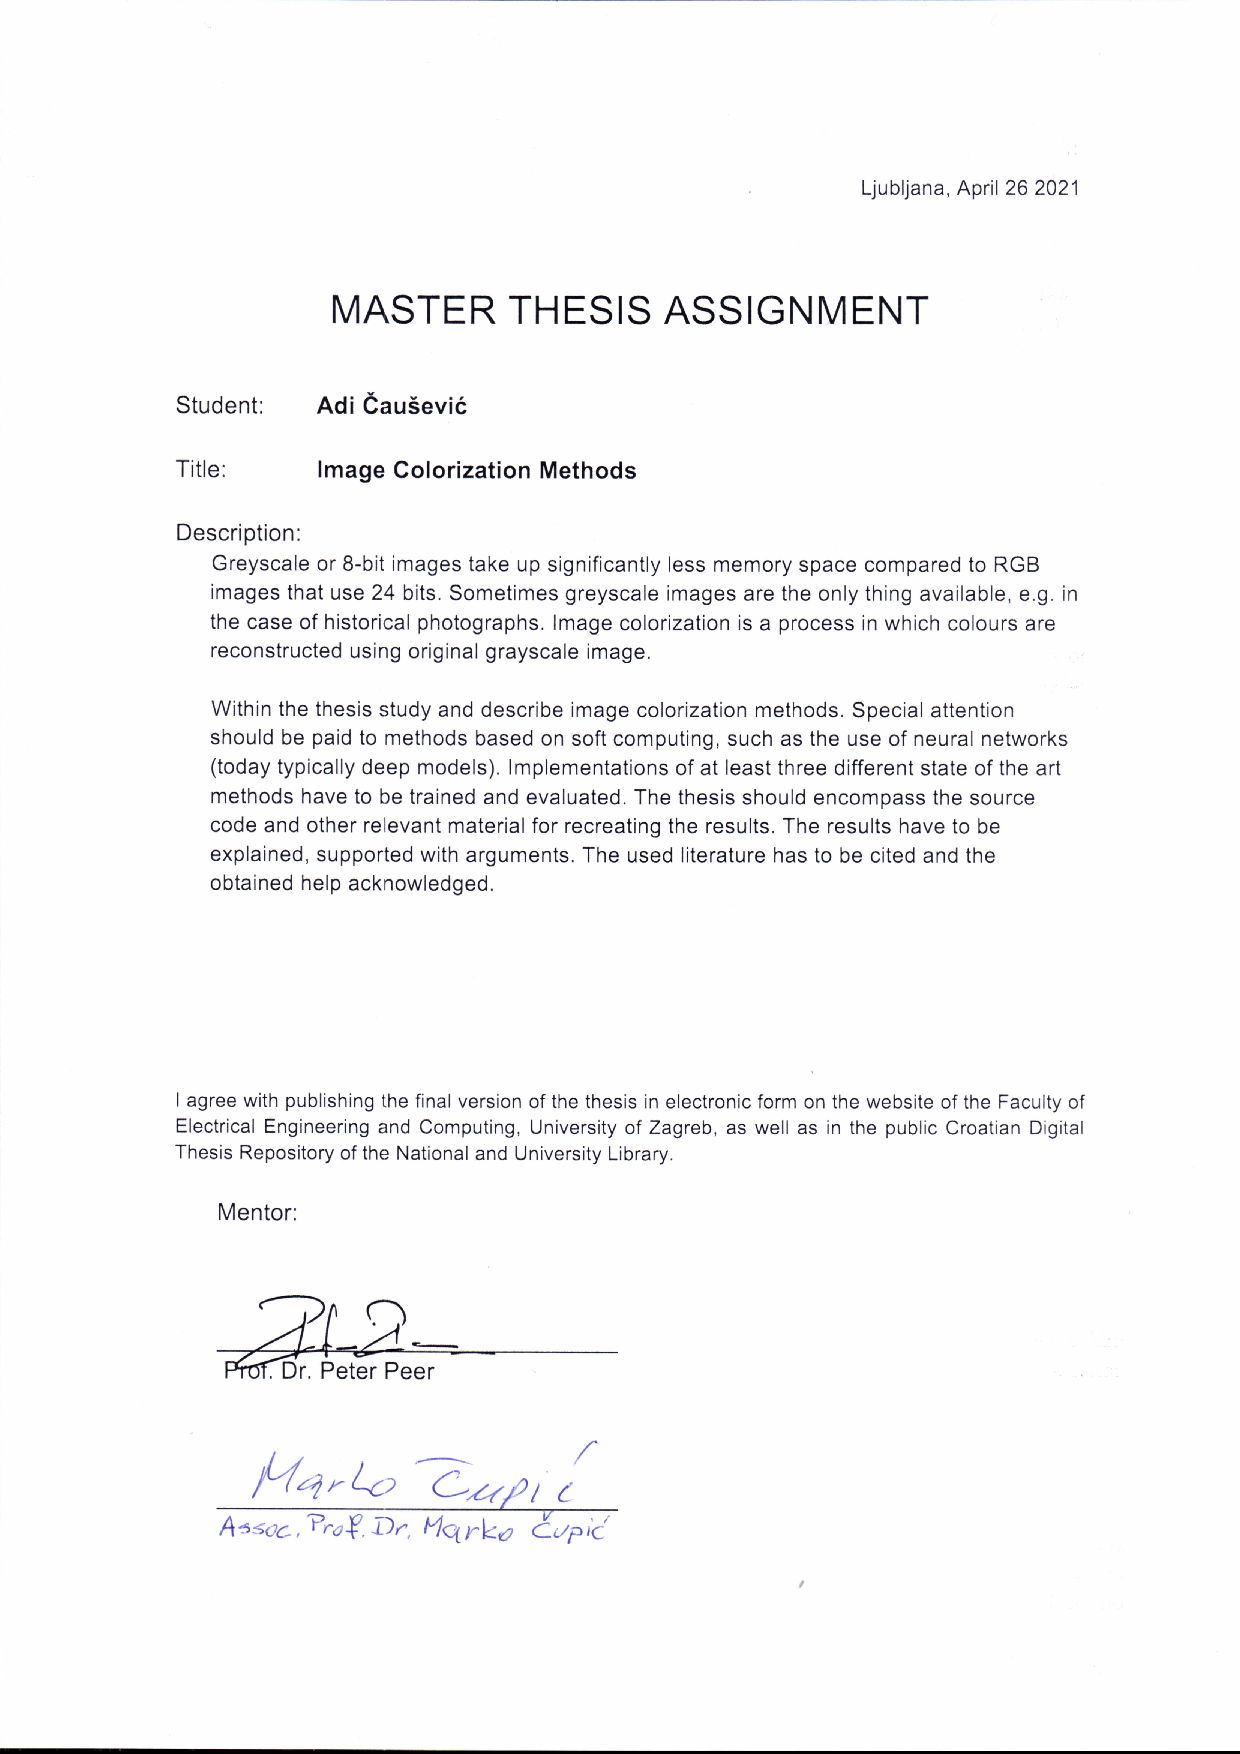
\includegraphics[width=1.\linewidth]{assignment}
\end{figure}

% Zahvala
\subfile{chapters/thanks}

% Table of contents
\tableofcontents

% Chapters
\subfile{chapters/introduction}
\subfile{chapters/base}
\subfile{chapters/models}
\subfile{chapters/related}
\subfile{chapters/conclusion}

% Bibliography
\bibliography{literatura}
\bibliographystyle{plainnat}

% Abstract
\subfile{chapters/abstract}

% Sazetak
\subfile{chapters/sazetak}
\end{document}
